%%%%%%%%%%%%%%%%%%%%%%%%%%%%%%%%%%%%%%%%%
% Programming/Coding Assignment
% LaTeX Template
%
% This template has been downloaded from:
% http://www.latextemplates.com
%
% Original author:
% Ted Pavlic (http://www.tedpavlic.com)
%
% Note:
% The \lipsum[#] commands throughout this template generate dummy text
% to fill the template out. These commands should all be removed when 
% writing assignment content.
%
% This template uses a Perl script as an example snippet of code, most other
% languages are also usable. Configure them in the "CODE INCLUSION 
% CONFIGURATION" section.
%
%%%%%%%%%%%%%%%%%%%%%%%%%%%%%%%%%%%%%%%%%

%----------------------------------------------------------------------------------------
%	PACKAGES AND OTHER DOCUMENT CONFIGURATIONS
%----------------------------------------------------------------------------------------

\documentclass{article}

\usepackage{fancyhdr} % Required for custom headers
\usepackage{lastpage} % Required to determine the last page for the footer
\usepackage{extramarks} % Required for headers and footers
\usepackage[usenames,dvipsnames]{color} % Required for custom colors
\usepackage{graphicx} % Required to insert images
\usepackage{subcaption}
\usepackage{listings} % Required for insertion of code
\usepackage{courier} % Required for the courier font
\usepackage{lipsum} % Used for inserting dummy 'Lorem ipsum' text into the template
\usepackage{amsmath}

% Margins
\topmargin=-0.45in
\evensidemargin=0in
\oddsidemargin=0in
\textwidth=6.5in
\textheight=9.0in
\headsep=0.25in

\linespread{1.1} % Line spacing

% Set up the header and footer
\pagestyle{fancy}
\lhead{\hmwkAuthorName} % Top left header
\chead{\hmwkClass\ (\hmwkClassTime): \hmwkTitle} % Top center head
%\rhead{\firstxmark} % Top right header
\lfoot{\lastxmark} % Bottom left footer
\cfoot{} % Bottom center footer
\rfoot{Page\ \thepage\ of\ \protect\pageref{LastPage}} % Bottom right footer
\renewcommand\headrulewidth{0.4pt} % Size of the header rule
\renewcommand\footrulewidth{0.4pt} % Size of the footer rule

\setlength\parindent{0pt} % Removes all indentation from paragraphs

%----------------------------------------------------------------------------------------
%	CODE INCLUSION CONFIGURATION
%----------------------------------------------------------------------------------------

\definecolor{MyDarkGreen}{rgb}{0.0,0.4,0.0} % This is the color used for comments
\lstloadlanguages{Perl} % Load Perl syntax for listings, for a list of other languages supported see: ftp://ftp.tex.ac.uk/tex-archive/macros/latex/contrib/listings/listings.pdf
\lstset{language=Perl, % Use Perl in this example
        frame=single, % Single frame around code
        basicstyle=\small\ttfamily, % Use small true type font
        keywordstyle=[1]\color{Blue}\bf, % Perl functions bold and blue
        keywordstyle=[2]\color{Purple}, % Perl function arguments purple
        keywordstyle=[3]\color{Blue}\underbar, % Custom functions underlined and blue
        identifierstyle=, % Nothing special about identifiers                                         
        commentstyle=\usefont{T1}{pcr}{m}{sl}\color{MyDarkGreen}\small, % Comments small dark green courier font
        stringstyle=\color{Purple}, % Strings are purple
        showstringspaces=false, % Don't put marks in string spaces
        tabsize=5, % 5 spaces per tab
        %
        % Put standard Perl functions not included in the default language here
        morekeywords={rand},
        %
        % Put Perl function parameters here
        morekeywords=[2]{on, off, interp},
        %
        % Put user defined functions here
        morekeywords=[3]{test},
       	%
        morecomment=[l][\color{Blue}]{...}, % Line continuation (...) like blue comment
        numbers=left, % Line numbers on left
        firstnumber=1, % Line numbers start with line 1
        numberstyle=\tiny\color{Blue}, % Line numbers are blue and small
        stepnumber=5 % Line numbers go in steps of 5
}

% Creates a new command to include a perl script, the first parameter is the filename of the script (without .pl), the second parameter is the caption
\newcommand{\perlscript}[2]{
\begin{itemize}
\item[]\lstinputlisting[caption=#2,label=#1]{#1.pl}
\end{itemize}
}

%----------------------------------------------------------------------------------------
%	DOCUMENT STRUCTURE COMMANDS
%	Skip this unless you know what you're doing
%----------------------------------------------------------------------------------------

% Header and footer for when a page split occurs within a problem environment
\newcommand{\enterProblemHeader}[1]{
%\nobreak\extramarks{#1}{#1 continued on next page\ldots}\nobreak
%\nobreak\extramarks{#1 (continued)}{#1 continued on next page\ldots}\nobreak
}

% Header and footer for when a page split occurs between problem environments
\newcommand{\exitProblemHeader}[1]{
%\nobreak\extramarks{#1 (continued)}{#1 continued on next page\ldots}\nobreak
%\nobreak\extramarks{#1}{}\nobreak
}

\setcounter{secnumdepth}{0} % Removes default section numbers
\newcounter{homeworkPartCounter} % Creates a counter to keep track of the number of problems
\setcounter{homeworkPartCounter}{0}

\newcommand{\homeworkPartName}{}
\newenvironment{homeworkPart}[1][Part \arabic{homeworkPartCounter}]{ % Makes a new environment called homeworkPart which takes 1 argument (custom name) but the default is "Problem #"
\stepcounter{homeworkPartCounter} % Increase counter for number of problems
\renewcommand{\homeworkPartName}{#1} % Assign \homeworkPartName the name of the problem
\section{\homeworkPartName} % Make a section in the document with the custom problem count
\enterProblemHeader{\homeworkPartName} % Header and footer within the environment
}{
\exitProblemHeader{\homeworkPartName} % Header and footer after the environment
}

\newcommand{\problemAnswer}[1]{ % Defines the problem answer command with the content as the only argument
\noindent\framebox[\columnwidth][c]{\begin{minipage}{0.98\columnwidth}#1\end{minipage}} % Makes the box around the problem answer and puts the content inside
}

\newcommand{\homeworkSectionName}{}
\newenvironment{homeworkSection}[1]{ % New environment for sections within homework problems, takes 1 argument - the name of the section
\renewcommand{\homeworkSectionName}{#1} % Assign \homeworkSectionName to the name of the section from the environment argument
\subsection{\homeworkSectionName} % Make a subsection with the custom name of the subsection
\enterProblemHeader{\homeworkPartName\ [\homeworkSectionName]} % Header and footer within the environment
}{
\enterProblemHeader{\homeworkPartName} % Header and footer after the environment
}

%----------------------------------------------------------------------------------------
%	NAME AND CLASS SECTION
%----------------------------------------------------------------------------------------

\newcommand{\hmwkTitle}{Project 3} % Assignment title
\newcommand{\hmwkDueDate}{Monday,\ March\ 19,\ 2018} % Due date
\newcommand{\hmwkClass}{CSC411} % Course/class
\newcommand{\hmwkClassTime}{L5101} % Class/lecture time
\newcommand{\hmwkAuthorName}{Anas Al-Raheem} % Your name

%----------------------------------------------------------------------------------------
%	TITLE PAGE
%----------------------------------------------------------------------------------------

\title{
\vspace{2in}
\textmd{\textbf{\hmwkClass:\ \hmwkTitle}}\\
\normalsize\vspace{0.1in}\small{Due\ on\ \hmwkDueDate}\\
\vspace{0.1in}
\vspace{3in}
}

\author{\textbf{\hmwkAuthorName}}
\date{\hmwkDueDate} % Insert date here if you want it to appear below your name

%----------------------------------------------------------------------------------------

\begin{document}

\maketitle
\clearpage
%----------------------------------------------------------------------------------------
%	Part 1 & 2
%----------------------------------------------------------------------------------------

% To have just one problem per page, simply put a \clearpage after each problem

\begin{homeworkPart}

The data-set consists of real and fake news headlines related to the recent U.S elections, with about 2000 real headline and about 1300 fake headlines. By looking at the number of word occurrences we see that the words used the most for both real and fake headlines are mostly similar. We can also see that many of those words are stop-words ("of", "for", "on" ... etc). I have listed below three examples that I believe will help in classifying the headlines as real or fake:\\

- "trumps" $\longrightarrow$ real : 219, fake:4\\
- "korea" $\longrightarrow$ real : 79, fake:0\\
- "turnbull" $\longrightarrow$ real:55, fake:0\\

\end{homeworkPart}
\begin{homeworkPart}

I tried to run the classification using m in the range 1 - 5, and for each value of m I tried $\hat p$ values in the range 0.01 - 0.1. I decided to use the m and $\hat p$ that resulted in the highest performance for both real and fake headlines when classifying the validation sets. The performance is below:
\begin{verbatim}
    training , for label: real , performance: 97.9680696662 %
    training , for label: fake , performance: 96.8131868132 %
    validation , for label: real , performance: 89.8305084746 %
    validation , for label: fake , performance: 83.5051546392 %
    test , for label: real , performance: 86.7796610169 %
    test , for label: fake , performance: 78.3505154639 %
\end{verbatim}

and the combined performance for both classes:
\begin{verbatim}
    training performance: 97.5087412587 %
    validation performance: 87.3210633947 %
    test performance: 83.4355828221 %
\end{verbatim}

when computing p(headline $\mid$ class) I used the following code (lst is a list of headline):
\begin{verbatim}
    for line in lst:
        line_words = list(set(line.split()))
        p_line_real = 0.
        p_line_fake = 0.

        for word in words_dict:
            if word in line_words:
                p_line_real += np.log(words_dict[word][1])
                p_line_fake += np.log(words_dict[word][0])
            else:
                p_line_real += np.log(1. -  (words_dict[word][1]))
                p_line_fake += np.log(1. -  (words_dict[word][0]))

        p_line_real = np.exp(p_line_real)
        p_line_fake = np.exp(p_line_fake)
\end{verbatim}
For each headline the code computes p(headline $\mid$ class), so for all words in training set, add up log(word count) if the word is present in headline, otherwise add log(1 - word count). And finally compute exp of that sum, the result can then be used to compute p(class $\mid$ headline).

\end{homeworkPart}
\clearpage
%----------------------------------------------------------------------------------------
%	Part 3 & 4
%----------------------------------------------------------------------------------------



\begin{homeworkPart}

A):\\
\begin{verbatim}
    part 3a: Words with stop words
    p(real|word) :
    [('korea', 0.9999984706460329), ('travel', 0.999998161452981), 
    ('turnbull', 0.9999979567576792), ('australia', 0.9999963593007417), 
    ('refugee', 0.999995744141818), ('paris', 0.9999957441414531), 
    ('debate', 0.9999948834115259), ('tax', 0.9999948834110846), 
    ('congress', 0.9999945147023779), ('defends', 0.9999945147023779)]
    p(fake|word) :
    [('star', 0.6503072189992896), ('black', 0.613751194679261), 
    ('breaking', 0.5849902550380285), ('u', 0.5689972950641514), 
    ('soros', 0.5517624714313497), ('won', 0.551762461072533), 
    ('woman', 0.5129396870889822), ('homeless', 0.4669787763834351), 
    ('info', 0.44067670120589464), ('daily', 0.41171181939951795)]
    p(real|!word) :
    [('star', 0.6022727278336234), ('black', 0.6022727277070424), 
    ('breaking', 0.6022727276231271), ('u', 0.60227272758131), 
    ('soros', 0.6022727275395864), ('won', 0.6022727275395864), 
    ('woman', 0.6022727274564178), ('homeless', 0.6022727273736188), 
    ('info', 0.6022727273323573), ('daily', 0.6022727272911872)]
    p(fake|!word) :
    [('trump', 0.3978205609714579), ('donald', 0.3977375161354875), 
    ('to', 0.3977307151974267), ('trumps', 0.39772921604346484), 
    ('in', 0.39772902488377293), ('us', 0.3977290177194766), 
    ('on', 0.3977287829191988), ('says', 0.397728749350079), 
    ('of', 0.3977286570848396), ('for', 0.39772865663446955)]
\end{verbatim}
For each of the above 4 lists, I calculated p(class$|$word) or p(class$|$!word) and select the top 10 words with the highest probability in each category. We can also see that the top 10 in p(fake$|$word) and p(real$|$!word) have the same words (but different probabilities). This makes sense as the words that most strongly indicate the headline is fake are the ones their absence most strongly indicates the headline is real. We can also notice that some words presence have a bigger effect on classifying headline than the effect of words being absent.\\

B):\\
\begin{verbatim}
    part 3b: Words without stop words
    p(real|word) :
    [('korea', 0.9999983302729929), ('travel', 0.999997992709485), 
    ('turnbull', 0.9999977692320788), ('australia', 0.9999960251985364), 
    ('refugee', 0.9999953535950954), ('paris', 0.9999953535946932), 
    ('debate', 0.9999944138877667), ('tax', 0.9999944138872799), 
    ('congress', 0.9999940113474387), ('defends', 0.9999940113474387)]
    p(fake|word) :
    [('star', 0.6699927149993263), ('black', 0.6343383147997317), 
    ('breaking', 0.6061271607440026), ('u', 0.5903786852821299), 
    ('soros', 0.5733580738326386), ('won', 0.5733580635116059), 
    ('woman', 0.5348294464171838), ('homeless', 0.48887646443934396), 
    ('info', 0.46241130985149403), ('daily', 0.4331244024846518)]
    p(real|!word) :
    [('star', 0.6022727279198156), ('black', 0.6022727277802438), 
    ('breaking', 0.6022727276877157), ('u', 0.6022727276416064), 
    ('won', 0.6022727275956004), ('soros', 0.6022727275956002), 
    ('woman', 0.6022727275038947), ('homeless', 0.6022727274125963), 
    ('info', 0.6022727273670989), ('daily', 0.6022727273217023)]
    p(fake|!word) :
    [('trump', 0.3978210132482278), ('donald', 0.397737612527062), 
    ('trumps', 0.3977292352835487), ('says', 0.39772876387319733), 
    ('clinton', 0.39772795488797064), ('election', 0.3977279457362376), 
    ('ban', 0.3977278461398317), ('korea', 0.39772780133436325), 
    ('north', 0.39772780128976093), ('president', 0.397727721530816)]
\end{verbatim}

C):\\
It would make sense to remove stop words as they are necessary words used in all sentences and they do not add any value in determining if a headline is real or fake. On the other hand It would make sense to keep them, as they help in identifying relations between headlines. For example if fake headlines has some specific patterns related to those stop words, we can detect this pattern and it will help us categorize the headlines. This is especially useful if many of the headlines have the same origin.

\end{homeworkPart}

\clearpage

\begin{homeworkPart}

\begin{figure*}[h!]
    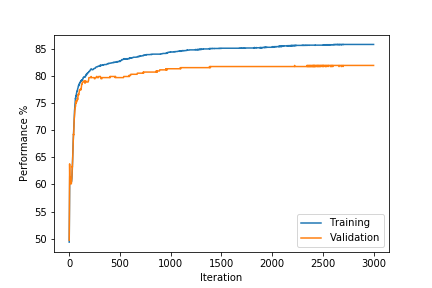
\includegraphics[scale=1]{part4_learning_curve.png}
    \caption{Learning Curve}
    \label{fig:Learning Curve}
\end{figure*}

For the L2 regularization, I tried different values for lambda, starting from 0.1 to 0.001. I noticed that for large values such as $0.1+$, the training performance would halt at about $80\%$ and for even larger values (like 0.5) the performance seems to fluctuate between $\sim80\%$ and $\sim40\%$. For small lambda values such as 0.001 over-fitting will still occur and the training performance will reach $\sim100\%$. I decided to use lambda = 0.05, which seemed to limit the training performance at $\sim85\%$ and still achieve a high performance for the validation set (for both validation and test sets  $\sim82\%$).

\end{homeworkPart}

\clearpage
%----------------------------------------------------------------------------------------
%	Part 5 & 6
%----------------------------------------------------------------------------------------

\begin{homeworkPart}

Naive Bayes:\\\\
$\theta_{0} = log(\frac{P(y = real)}{P(y = fake)}) - \sum_{j} log(\frac{P(x_j = 0 | y = real)}{P(x_j = 0 | y = fake)})$\\\\
$\theta_{i\neq0} = log(\frac{P(I_i(x) = 1 | y = real)}{P(I_i(x) = 1 | y = fake)}) - log(\frac{P(I_i(x) = 0 | y = real)}{P(I_i(x) = 0 | y = fake)})$\\\\
Logistic Regression:\\\\
$\theta_{0} = bias$\\\\
$\theta_{i\neq0} = [(y = fake) * log(P(y = fake | I_i(x), \theta_i))] + [(y = real) * log(P(y = real | I_i(x), \theta_i))]$\\\\
$ \Longrightarrow \theta_{i\neq0} = [(y = fake) * log(\frac{1}{1 + exp(-\theta_i^T I_i(x))})] + [(y = real) * log(\frac{exp(-\theta_i^T I_i(x))}{1 + exp(-\theta_i^T I_i(x))})]$\\\\
In both cases the $I_i$ is a function that indicate if word i is part of the headline:\\
$I_i(x)= 
\begin{cases}
    1,              & \text{if word i exists in the headline} \\
    0,              & \text{otherwise}
\end{cases}$

\end{homeworkPart}

\begin{homeworkPart}

A):\\
\begin{verbatim}
    top 10 positive real thetas:
    [('trumps', 0.6948395), ('donald', 0.5091938), ('us', 0.35595533), 
    ('says', 0.29129344), ('trump', 0.28825286), ('turnbull', 0.1987107), 
    ('korea', 0.18613984), ('north', 0.18608509), ('ban', 0.17993604), 
    ('travel', 0.14982505)]
    top 10 positive fake thetas:
    [('hillary', 0.42983687), ('the', 0.38218454), ('just', 0.2566552), 
    ('that', 0.23291568), ('will', 0.21895349), ('by', 0.21495272), 
    ('is', 0.21359529), ('watch', 0.2083732), ('are', 0.19982328), 
    ('if', 0.19676395)]
    top 10 negative real thetas:
    [('hillary', -0.42981833), ('the', -0.38219044), ('just', -0.25664032), 
    ('that', -0.23293833), ('will', -0.21896851), ('by', -0.21493603), 
    ('is', -0.21360353), ('watch', -0.20834945), ('are', -0.1998357), 
    ('if', -0.19674894)]
    top 10 negative fake thetas:
    [('trumps', -0.6948333), ('donald', -0.50920653), ('us', -0.35595867), 
    ('says', -0.29130432), ('trump', -0.28825775), ('turnbull', -0.19872041), 
    ('korea', -0.18613791), ('north', -0.18606757), ('ban', -0.17994043), 
    ('travel', -0.14981394)]
\end{verbatim}
We are running logistic regression for two classes and thus we have two sets of weights, one representing the class real and the other for class fake. I selected the top 10 positive and negative thetas from each weight set. We can see that the top 10 positives for one class are the same as the top 10 negative for the other class. This makes sense as the words that strongly indicate a headline belongs to some class c are also the ones that will indicate a headline belongs to another class not c if they are absent from the headline.\\
We can see that there are similar words in this part to the words from part 3(a). All the words in the top 10 positive real thetas are found in part 3(a) (none for top 10 positive fake thetas).\\

B):\\
\begin{verbatim}
    part 6b: top 10 positive and negative thetas without stop words
    top 10 positive real thetas:
    [('trumps', 0.6948395), ('donald', 0.5091938), ('says', 0.29129344), 
    ('trump', 0.28825286), ('turnbull', 0.1987107), ('korea', 0.18613984), 
    ('north', 0.18608509), ('ban', 0.17993604), ('travel', 0.14982505), 
    ('climate', 0.14284052)]
    top 10 positive fake thetas:
    [('hillary', 0.42983687), ('just', 0.2566552), ('watch', 0.2083732), 
    ('victory', 0.17650263), ('star', 0.1754553), ('america', 0.16210474), 
    ('win', 0.15329543), ('breaking', 0.14730132), ('black', 0.14662313), 
    ('voter', 0.13826963)]
    top 10 negative real thetas:
    [('hillary', -0.42981833), ('just', -0.25664032), ('watch', -0.20834945), 
    ('victory', -0.17649065), ('star', -0.17543143), ('america', -0.16211958), 
    ('win', -0.15332834), ('breaking', -0.14730439), ('black', -0.14663115), 
    ('voter', -0.1382601)]
    top 10 negative fake thetas:
    [('trumps', -0.6948333), ('donald', -0.50920653), ('says', -0.29130432), 
    ('trump', -0.28825775), ('turnbull', -0.19872041), ('korea', -0.18613791), 
    ('north', -0.18606757), ('ban', -0.17994043), ('travel', -0.14981394), 
    ('climate', -0.14283024)
\end{verbatim}
We can see that there are many similar words in this part to the words from part 3(b). most the words in the top 10 positive real thetas are found in part 3(a) (and some words from top 10 positive fake thetas).\\

C):\\
Deciding importance based on the magnitude could be a bad idea, because if all the thetas are not normalized than some thetas might be more important than others but they might still have less magnitude than those other thetas.\\
It is reasonable to use the magnitude in our case because the thetas are normalized by the size of the training set. Also because when trying to determine a class of a headline, the thetas capture the magnitude of effects different words have on determining the classification. 

\end{homeworkPart}
\clearpage

%----------------------------------------------------------------------------------------
%	Part 7 & 8
%----------------------------------------------------------------------------------------

\begin{homeworkPart}

A):\\

I used the following code to decide which depth to use:
\begin{verbatim}
    depths = [10, 25, 50, 75, 100, 125, 150, 175, 200, 250]
    for depth in depths:
        np.random.seed(0)
        dtc = tree.DecisionTreeClassifier(max_depth=depth, max_features=0.7)
        dtc.fit(training_x, training_y)

        print "Depth: ", depth
        print "training performance: ", 
            dtc.score(training_x, training_y) * 100, "%"
        print "validation performance: ", 
            dtc.score(validation_x, validation_y) * 100, "%"
\end{verbatim}
The results are: 
\begin{verbatim}
    Depth:  10
    training performance:  76.57342657342657 %
    validation performance:  72.1881390593047 %
    Depth:  25
    training performance:  88.1555944055944 %
    validation performance:  76.48261758691206 %
    Depth:  50
    training performance:  94.18706293706293 %
    validation performance:  78.11860940695297 %
    Depth:  75
    training performance:  97.2027972027972 %
    validation performance:  77.0961145194274 %
    Depth:  100
    training performance:  98.29545454545455 %
    validation performance:  79.55010224948876 %
    Depth:  125
    training performance:  99.38811188811188 %
    validation performance:  78.7321063394683 %
    Depth:  150
    training performance:  100.0 %
    validation performance:  78.11860940695297 %
    Depth:  175
    training performance:  100.0 %
    validation performance:  78.11860940695297 %
    Depth:  200
    training performance:  100.0 %
    validation performance:  78.11860940695297 %
    Depth:  250
    training performance:  100.0 %
    validation performance:  78.11860940695297 %
\end{verbatim}
I decided to choose depth 100, as it seemed to have the best performance on the validation set.\\

I also tried changing some of the default parameters and I noticed that changing max\_features to 0.7 was most beneficial, and it slightly improved the performance on the validation set (by about $2\%$). I tried different values for max\_features and run the code sample above to determine which value works best.

Performance on training set: $98.29545454545455\%$, and validation set: $79.55010224948876\%$.\\

B):\\
The program saves the graph as a tree.dot file, I used an online resource (http://webgraphviz.com/) to visualize that file:\\

\begin{figure*}[h!]
    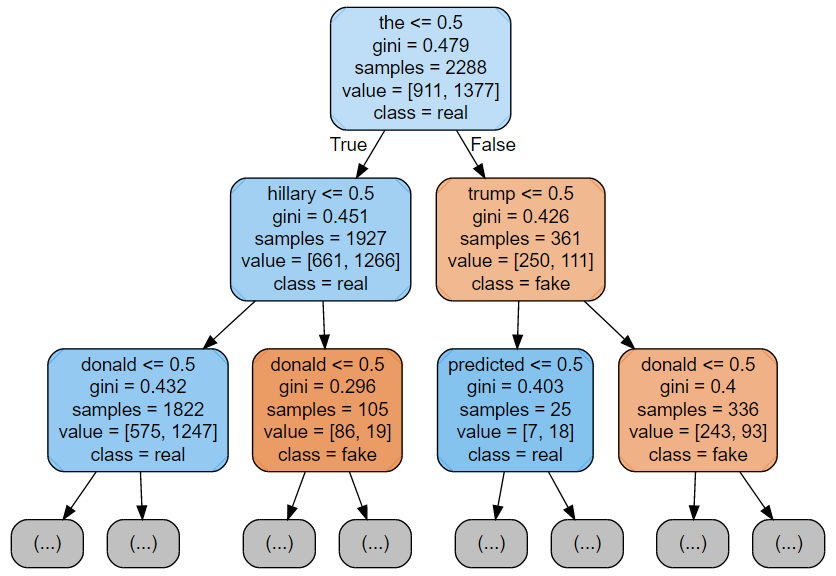
\includegraphics[scale=0.75]{tree.png}
    \caption{Decision Tree}
    \label{fig:Decision Tree}
\end{figure*}

We can see from the graph that some of the words are the same as the ones from part 3a and 6a, while others (like the top word "the") were not among the results of part 3a or part 6a.\\

C):\\

Naive Bayes performance:\\
- training performance: 97.5087412587 \%\\
- validation performance: 87.3210633947 \%\\
- test performance: 83.4355828221 \%\\

Logistic Regression performance:\\
- training performance: 85.88286713286713 \%\\
- validation performance: 82.0040899795501 \%\\
- test performance: 82.0040899795501 \%\\

Decision Tree performance:\\
- training performance:  98.29545454545455 \%\\
- validation performance:  79.55010224948876 \%\\
- test performance:  77.0961145194274 \%\\


Based on the performance on validation and test sets we can see that Naive Bayes performed the best, while Decision Tree performed the worst. We can also see based on the training set performance that the Decision Tree over-fitted the most, while logistic regression over-fitted the least. 


\end{homeworkPart}

\begin{homeworkPart}

A):\\
I used the following functions:
\begin{verbatim}
def get_mutual_information(p_fake, p_real, real_train, fake_train, x):
    train_dict = {}
    train_dict = get_counts(real_train, 1, train_dict)
    train_dict = get_counts(fake_train, 0, train_dict)

    p_x = (train_dict[x][0] + train_dict[x][1]) / 
            float(len(real_train) + len(fake_train))
    h_x = (- p_x * np.log2(p_x)) + (- (1. - p_x) * np.log2(1. - p_x))
    
    m = 1.
    p = 0.03
    train_dict = {}
    train_dict = get_counts(real_train, 1, train_dict)
    train_dict = get_counts(fake_train, 0, train_dict)

    for k, v in train_dict.items():
        train_dict[k][0] = (train_dict[k][0] + m * p) / (float(len(fake_train)) + m)
        train_dict[k][1] = (train_dict[k][1] + m * p) / (float(len(real_train)) + m)

    p_word_real, p_word_fake, p_not_word_real, 
                    p_not_word_fake = get_word_p(x, train_dict)

    h_x_given_y = (p_fake * - ( (p_not_word_fake * np.log2(p_not_word_fake)) 
                                + (p_word_fake * np.log2(p_word_fake)) )) \
                  + (p_real * - ( (p_not_word_real * np.log2(p_not_word_real)) 
                                    + (p_word_real * np.log2(p_word_real)) ))

    I_Y_x = h_x - h_x_given_y
    
    return I_Y_x


def get_word_p(x, words_dict):
    p_word_real = 0.
    p_word_fake = 0.
    for word in words_dict:
        if word == x:
            p_word_real += np.log(words_dict[word][1])
            p_word_fake += np.log(words_dict[word][0])
        else:
            p_word_real += np.log(1. -  (words_dict[word][1]))
            p_word_fake += np.log(1. -  (words_dict[word][0]))

    p_word_real = np.exp(p_word_real)
    p_word_fake = np.exp(p_word_fake)

    p_not_word_real = 1. - p_word_real
    p_not_word_fake = 1. - p_word_fake
    
    return p_word_real, p_word_fake, p_not_word_real, p_not_word_fake
\end{verbatim}
The top most split uses the word 'the' and so I ran the function:
\begin{verbatim}
     I_x_i = get_mutual_information(p_fake, p_real, real_train, fake_train, "the")
\end{verbatim}
the result: I(Y, 'the') = 0.6289108057043181\\

B):\\

I chose the word 'hillary', the same code as in part 8a is used:
\begin{verbatim}
     I_x_j = get_mutual_information(p_fake, p_real, real_train, fake_train, "hillary")
\end{verbatim}

the result: I(Y, 'hillary') = 0.2985153264875215\\

We can see that the result differ a lot, which signifies the importance of word 'the' in determining the class in comparison with the word 'hillary'. 

\end{homeworkPart}

\clearpage

%----------------------------------------------------------------------------------------

\end{document}